\section{Nico Ekklesia Sembiring (1174096)}
\subsection{Pengertian}
Sistem Informasi Geografis terdiri atas 3 kata. Yaitu Sistem, Informasi, dan Geografis. \hfill\break
SISTEM\hfill\break
Pada umumnya sistem diartikan sebagai suatu kesatuan yang terdiri atas komponen maupun elemen yang saling berinteraksi, saling berkaitan, atau saling bergantung sehingga membentuk keseluruhan yang kompleks.\hfill\break
INFORMASI\hfill\break
Informasi merupakan bentuk data yang telah diproses menjadi bentuk yang memiliki arti bagi penerima dan dapat berupa fakta, suatu nilai yang bermanfaat. Pada bagian ini ada suatu proses transformasi data menjadi suatu informasi yaitu input- proses -output.\hfill\break
GEOGRAFI\hfill\break
Geografi adalah ilmu yang mempelajari tentang lokasi serta persamaan dan perbedaan variasi keruangan atas fenomena fisik dan manusia di atas permukaan bumi. Geografi memiliki definisi lain yaitu ilmu yang mempelajari perbedaan dan persamaan terhadap fenomena yang terjadi pada geosfer melalui sudut pandang kewilayahan dan lingkungan dalam konteks keruangan.\hfill\break
SISTEM INFORMASI\hfill\break
Pada umumnya sistem informasi diartikan sebagai suatu sistem terintegrasi yang dapat menyediakan informasi yang bermanfaat untuk kepentingan pengguna, untuk menyediakan informasi untuk mendukung operasi, manajemen dalam suatu organisasi. Sistem ini memanfaatkan perangkat keras dan perangkat lunak komputer, prosedur manual, model manajemen dan basis data\hfill\break
SISTEM INFORMASI GEOGRAFIS\hfill\break
Pengertian dari Sistem Informasi Geografis (GIS) pada umumnya adalah sistem informasi khusus yang digunakan untuk melakukan pengelolaan data yang memiliki informasi geospasial. SIG juga merupakan sejenis perangkat lunak yang dapat digunakan untuk pemasukan, penyimpanan, manipulasi, menampilkan, dan keluaran informasi geografis berikut atribut – atributnya. SIG biasa digunakan untuk memberi nilai, dengan cara melakukan pengaturan dan memperlihatkan data secara tepat, menggabungkan dengan data lain, melakukan analisis terhadap data, dan menghasilkan data baru yang berguna, pada gilirannya SIG dapat membantu untuk pengambilan keputusan. Sistem Informasi Geografi dibagi menjadi dua kelompok yaitu sistem manual (analog), dan sistem otomatis (yang berbasis digital komputer). Perbedaan yang paling mendasar terletak pada cara pengelolaannya.\hfill\break

\subsection{Sejarah}
Sejarah GIS dimulai dari awal tahun 1960-an dimana terjadi perkembangan yang semakin pesat dalam ilmu komputer sehingga siap untuk digunakan pada bidang lain di luar militer. Ahli meteorologi, geologi, dan geofisika mulai menggunakan teknologi komputer dalam , melakukan pembuatan peta.\hfill\break
Pada tahun 1963 di Kanada terbentuk CGIS (Canadian Geographic Information System), dan selanjutnya menjadi SIG pertama di dunia. Kemudian 2 tahun setelahnya di Amerika Serikat dioperasikan sistem serupa yang bernama MIDAS yang biasa digunakan untuk memproses data-data sumber daya alam.\hfill\break
Seiring dengan berkembangnya teknologi, GIS juga mengalami perubahan ke arah yang lebih baik. \hfill\break
Berikut ini merupakan sejarah perkembangan GIS dari waktu ke waktu :\hfill\break
\begin{itemize}
	\item Pada 35000 tahun yang lalu, para pemburu Cro-Magnon menggambar hewan mangsa mereka di dinding gua Lascaux, Perancis, tidak hanya hewan mangsa, tetapi juga garis yang dipercaya sebagai rute migrasi hewan-hewan tersebut. Catatan penemuan awal ini sejalan dengan dua elemen struktur pada sistem informasi gegrafis modern sekarang ini, arsip grafis yang terhubung ke database atribut.\hfill\break
	\item Pada tahun 1700-an mulai diterapkan teknik survey modern untuk pemetaan topografis, penerapan ini termasuk juga versi awal pemetaan tematis, misalnya untuk keilmuan atau data sensus.\hfill\break
	\item Pada awal abad ke-20 diperlihatkan pengembangan “litografi foto” dimana peta tersebut dipisahkan menjadi beberapa lapisan (layer). Perkembangan perangkat keras komputer yang dipacu oleh penelitian senjata nuklir membawa aplikasi pemetaan menjadi multifungsi pada awal tahun 1960-an.\hfill\break
	\item Awal pengembangan SIG dimana mulai diterapkan di Ottawa, Ontario oleh Departemen Energi, Pertambangan dan Sumber Daya terjadi pada Tahun 1967.  Sistem ini dikembangkan oleh Roger Tomlinson, yang kemudian disebut sebagai CGIS (Canadian GIS – SIG Kanada),  sistem ini biasa digunakan untuk menyimpan, menganalisis dan mengolah data yang dikumpulkan dalam rangka kegiatan Inventarisasi Tanah Kanada (CLI – Canadian land Inventory). Hal ini merupakan sebuah inisiatif yang dilakukan mengetahui kemampuan suatu lahan di wilayah pedesaan Kanada dengan melakukan pemetaan berbagai informasi pada tanah, pertanian, pariwisata, alam bebas, unggas dan penggunaan tanah pada skala 1:250000. Faktor pemeringkatan klasifikasi juga diterapkan untuk keperluan analisis.\hfill\break
	\item GIS dengan gvSIG.CGIS merupakan sistem pertama di dunia dimana sistem ini merupakan hasil dari perbaikan yang sebelumnya telah memiliki, penghitungan, kemampuan timpang susun (overlay), pendigitalan/pemindaian (digitizing/scanning), mendukung sistem koordinat national yang terbentang di atas wilayah benua Amerika ,  hingga memasukkan garis dalam sebagai arc yang memiliki topologi dan menyimpan atribut dan informasi lokasional pada berkas terpisah. p, seorang geografer bernama Roger Tomlinson kemudian disebut “Bapak SIG”.\hfill\break
	\item CGIS bertahan sampai tahun 1970-an dan memakan waktu lama untuk penyempurnaan setelah pengembangan awal, dan tidak bisa bersaing denga aplikasi pemetaan komersil yang dikeluarkan beberapa vendor seperti Intergraph. Perkembangan perangkat keras mikro komputer memacu vendor lain seperti ESRI dan CARIS berhasil membuat banyak fitur SIG, menggabung pendekatan generasi pertama pada pemisahan informasi spasial dan atributnya, dengan pendekatan generasi kedua pada organisasi data atribut menjadi struktur database. Terjadinya perkembangan teknologi industri pada tahun 1980-an dan 1990-an memacu lagi pertumbuhan SIG pada workstation UNIX dan komputer pribadi. Pada akhir abad ke-20,  terjadi pertumbuhan yang cepat pada berbagai sistem yang dikonsolidasikan dan distandarisasikan menjadi platform lebih sedikit, serta para pengguna mulai mengekspor menampilkan data SIG lewat internet, yang membutuhkan standar pada format data dan transfer.
\end{itemize}
\subsection{Koordinat}
Untuk menggambarkan permukaan bumi yang berbentuk seperti bola ke dalam bentuk peta, diperlukan sebuah persamaan matematis yang dapat membantu mentransformasikan gambaran permukaan bumi. Persamaan ini disebut dengan sistem koordinat. Koordinat merupakan ciri khas utama dari GIS karena sistem koordinat ini yang dapat menunjukkan referensi geografis pada data data GIS. Dapat dikatakan bahwa sistem koordinat merupakan suatu pendekatan dalam mendefenisikan posisi data data GIS diatas permukaan bumi.\hfill\break
Dalam sistem koordinat, posisi objek pada permukaan bumi didefinisikan berdasarkan garis lintang(latitude) dan garis bujur(longitude). Garis lintang merupakan garis horizontal yang mengukur sudut antara satu titik dengan garis equator(garis khatulistiwa). Sedangkan garis bujur merupakan garis vertical yang mengukur sudut suatu titik dengan titik nol bumi, yaitu Greenwich Meridian, London\hfill\break
\begin{figure}[H]
	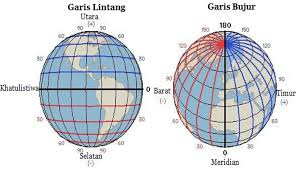
\includegraphics[width=4cm]{figures/1174096/1/koordinat2.jpg}
	\centering
	\caption{koordinat}
\end{figure}
Garis lintang terbagi menjadi 2, yaitu lintang utara dan lintang selatan dan garis bujur terbagi menjadi bujur timur dan bujur barat. Adanya kombinasi antara garis lintang dan garis bujur membentuk suatu koordinat lokasi di permukaan bumi dengan garis lintang sebagai sumbu x dan garis bujur sebagai sumbu y jika digambarkan dalam koordinat kartesius.
\begin{figure}[H]
	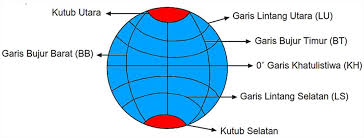
\includegraphics[width=4cm]{figures/1174096/1/lintangbujur.jpg}
	\centering
	\caption{garis lintang dan garis bujur}
\end{figure}
\begin{figure}[H]
	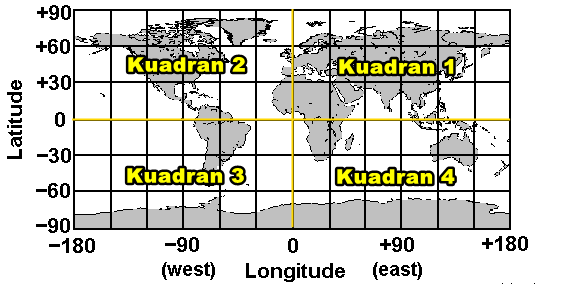
\includegraphics[width=4cm]{figures/1174096/1/Lintangbujurkuadran.png}
	\centering
	\caption{koordinat kartesius}
\end{figure}
\subsection{Data Geospasial}
Data Geospasial adalah data tentang aspek fisik dan administratif dari sebuah objek geografis.\hfill\break
Aspek fisik yang dimaksud mencakup bentuk anthropogenic dan bentuk alam baik yang terdapat di permukaan maupun di bawah permukaan bumi. Bentuk anthropogenic mengandung di dalamnya fenomena budaya seperti jalan, rel kereta api, bangunan, jembatan, dan sebagainya. Bentuk alam tentu saja adalah sungai, danau, pantai, daratan tinggi, dan sebagainya. \hfill\break
\begin{figure}[H]
	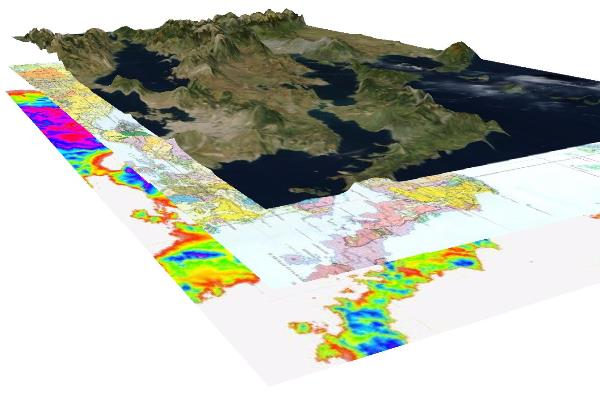
\includegraphics[width=4cm]{figures/1174096/1/consult_3.jpg}
	\centering
	\caption{aspek fisik}
\end{figure}
Sedangkan aspek administratif adalah pembagian atau pembatasan sosio-kultural yang dibuat oleh suatu organisasi atau badan untuk keperluan pengaturan dan pemakaian sumberdaya alam. Hal lain yang digolongkan kedalam aspek administratif ini adalah batas negara, zona, pembagian wilayah administrasi, kode pos, batas kepemilikan tanah, dan sebagainya.\hfill\break
\begin{figure}[H]
	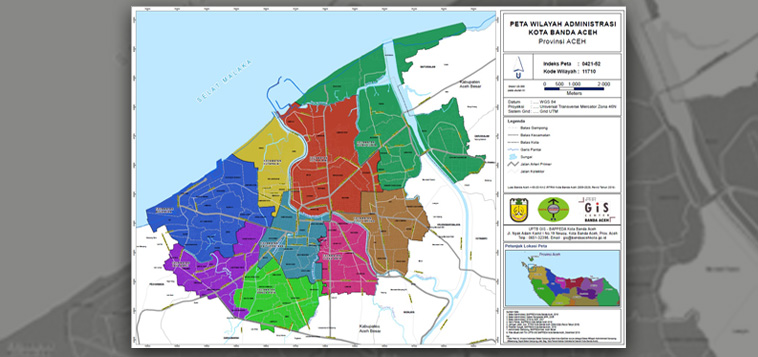
\includegraphics[width=4cm]{figures/1174096/1/PETA.jpg}
	\centering
	\caption{aspek administratif}
\end{figure}
Terdapat dua metode yang pada umumnya digunakan untuk menampilkan fitur geografis ke dalam GIS atau Sistem Informasi Geografis.\hfill\break 
\begin{itemize}
	\item Pertama, dengan struktur data vektor (vector data structure) yang terdiri dari sebuah gambaran titik geografis, baik yang berupa tanda titik, garis, maupun poligon. Struktur data vector biasa digunakan untuk menampilkan secara terpisah fitur geografis seperti batas administratif, jalan, bangunan, dan sungai. Sebuah objek grafis biasanya dikaitkan dengan informasi yang mengandung penjelasan tentang atribut objek itu, dan informasi ini bisa saja disimpan di dalam berkas spreadsheets atau pangkalan data terpisah.\hfill\break
	\item Kedua, dengan struktur data raster (raster data structure), terdiri dari serangkaian sel atau pixels yang biasa dipakai untuk menggambarkan data gambar sebagai data yang berkesinambungan. Dalam struktur data yang demikian, ada unsur resolusi sebagai ukuran dari dimensi fitur geografis yang terwakili dalam bentuk pixel. Biasanya data raster ini dipakai untuk citra satelit, ortografi digital, model elevasi digital (digital elevation models, DEM), peta digital, dan sebagainya.
\end{itemize}
\begin{figure}[H]
	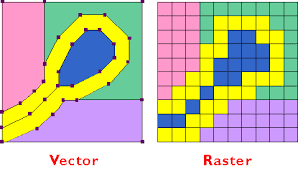
\includegraphics[width=4cm]{figures/1174096/1/vektordanraster.png}
	\centering
	\caption{data vektor dan raster}
\end{figure}
\subsection{Link}
\href{https://youtu.be/94y4uCmKc1Q}{Untuk selengkapnya lihat disini}

\subsection{Plagiarism}
\begin{figure}[H]
	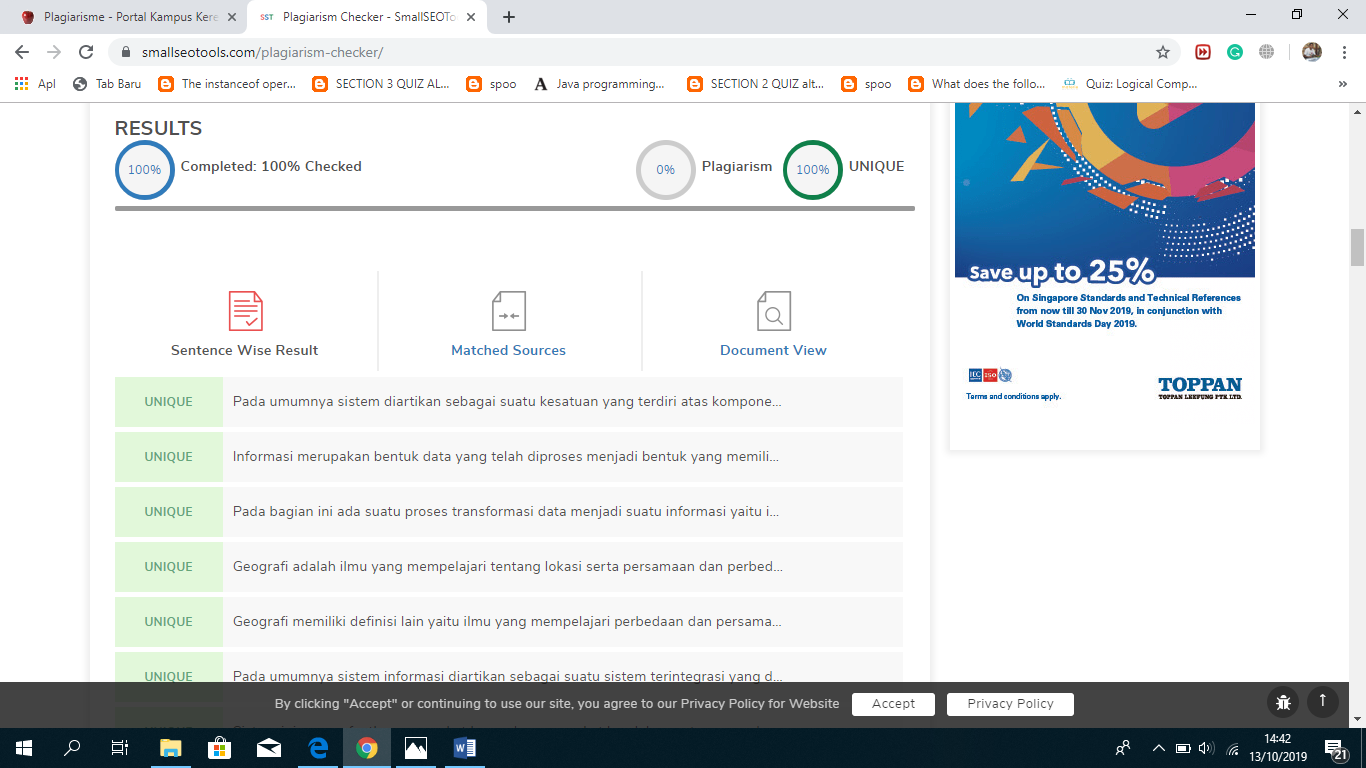
\includegraphics[width=4cm]{figures/1174096/1/plagiarisme.png}
	\centering
	\caption{cek plagiarisme}
\end{figure}


\subsection{Cara Penggunaan}
\subsubsection{Gambar}

\hfill\break

Contoh Gambar
\begin{figure}[H]
	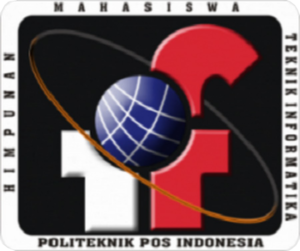
\includegraphics[width=4cm]{figures/himatif.png}
	\centering
	\caption{Contoh gambar.}
\end{figure}

\subsubsection{List}
\begin{enumerate}
	\item Satu
	\item Dua
\end{enumerate}

\begin{itemize}
	\item Satu
	\item Dua
\end{itemize}

\href{link kamu}{alias}
contoh link
\href{https://www.google.com/}{klik me}